\chapter{Thermovoltage, conductance and\\ behavior modeling}
\label{ch:vtp_g_model}


We now turn to the thermopower (thermovoltage) measurements and its modeling. As we have already discussed Kobayakawa, et al. \cite{kobayakawa2013diffusion} work presented results for even filling factors and low mobility samples measured at quite high frequencies. Our approach is much conservative. As shown in figure \ref{fig:setupVtpG}.

\begin{figure}
    \centering
    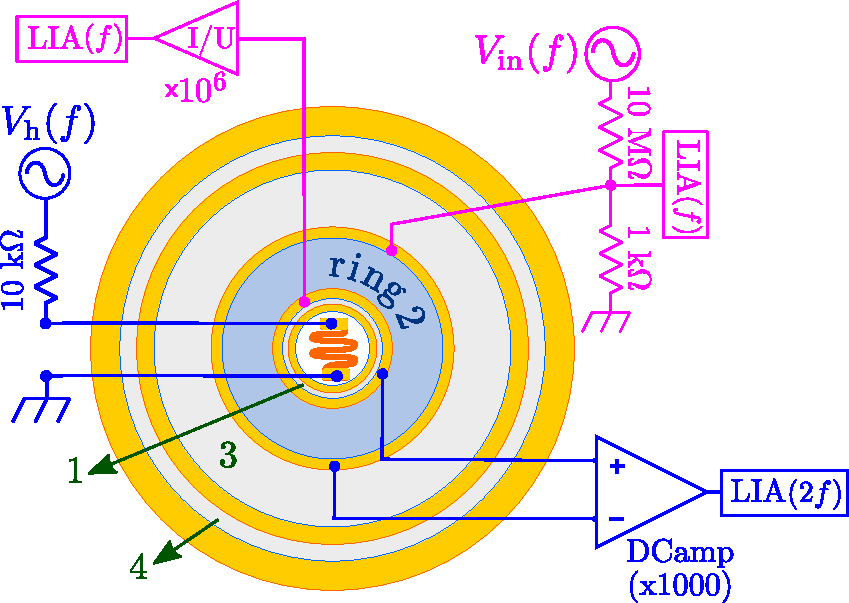
\includegraphics[width = 0.7\textwidth]{figures/vtpGmodel/setup_vtp_g.pdf}
    \caption{Experimental arrangement for the termovoltage (blue) and conductance (pink) measurements. Labels of rings are indicated. The radius of the outermost Corbino is \SI{1650}{\micro\meter}}
    \label{fig:setupVtpG}
\end{figure}

We heat the system by means of the resistive central heater, resulting in a thermovoltage at each Corbino ring. Each of them act independently, 

In order to produce the thermovoltage measurements different configurations were tested. The main problem here being the QH state its conductivity will be competing to the one of the measurement system. To make a proper measurement we must ensure a negligible current, i.e. a measurement system as ideal as possible having the highest possible input impedance. During initial measurements at INTI this became 



Here we will discuss and develop the model we obtained to describe the system and its different behaiviours. In the rest of this discussion it is important to keep in mind the two very different behaiviours of the system:
\begin{enumerate}
    \item Semi-filled Landau Levels (LL), magnetic field around half fractional filling factors $ \nu $ will present metal-like behaivour.
    \item Mobility gap, magnetic fields around integral fillig factors.
\end{enumerate}

We shall discuse them with kind of different aproaches. And we will also consider two dinsctinct behaiviours between low and high magnetic fields. A best definition is given afterwards, but they will be bassically distiguish by the field at which spin splitting in the conductance measurements are found,  in this particular samples $B \approx 1$.

\textcolor{red}{en la parte de caclulo de incerteza del modelo (determinación de $\Delta T$ meter cita a \cite{gum2008, gumModels}}.

\begin{figure}
    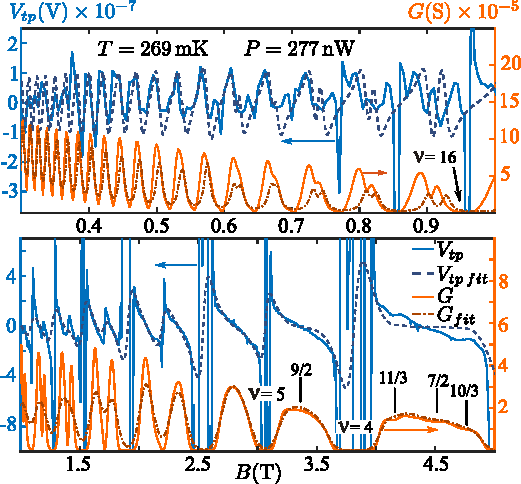
\includegraphics[width = 0.7\textwidth]{figures/vtpGmodel/termovoltageConductance/fig2.pdf}
    \caption{Conductance $G$ and thermovoltage $V_{tp}$ as a function of the magnetic field $B$ for \textit{ring 2} in Fig.~\ref{fig:corbino_exp_setup} at temperature $T$ with power $P$ supplied at the heater.
    Experimental data is plotted in solid lines. Theoretical (dashed) plots  are based on the calculation of 
    \textcolor{red}{eq.~(\ref{onsa})} 
    with the inferred transmission function as explained in (i) and (ii) for the upper and lower panel, respectively.  }
    \label{fig:lowHifield}
\end{figure}


\begin{figure}
    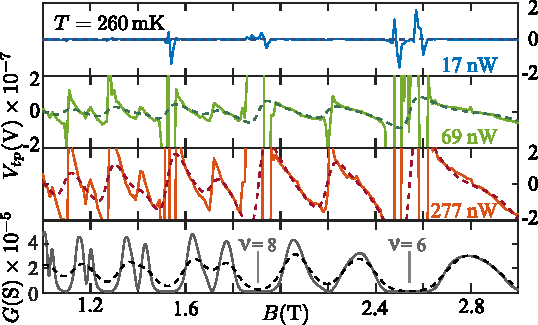
\includegraphics[width=0.7\textwidth]{figures/vtpGmodel/termovoltageConductance/fig3.pdf}
    \caption{Thermovoltage $V_{tp}$  for a fixed temperature and different powers $P^{\prime}$
    applied at the heater, assuming $\Delta T (P^{\prime}) = P^{\prime}/P \, \SI{1.08}{\milli\kelvin}$.
    $P$ and other details are the same as in  Fig.~\ref{fig:lowHifield}.}
    \label{fig:modelHeaterPower}
\end{figure}




\section{Thermoelectric performance}

\begin{figure}
    \centering
    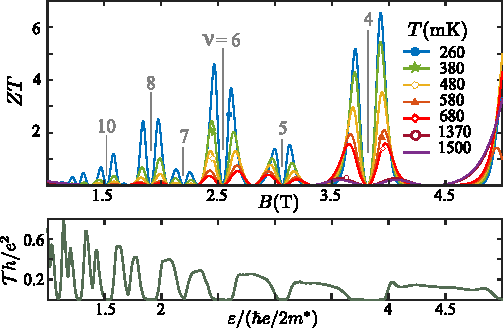
\includegraphics[width=0.7\textwidth]{figures/vtpGmodel/termovoltageConductance/fig5.pdf}
    \caption{Bottom: Transmission function ${\cal T}(\varepsilon)$. Top: Electron contribution to the figure of merit $ZT$.}
    \label{fig:ZT}
\end{figure}
The quality of the thermoelectric performance is evaluated in terms of
the efficiency (for the heat engine), 
 or coefficient of performance (for the refrigerator), which can be parameterized by the figure of merit \cite{benenti2016thermal,benenti2017fundamental}, $ZT = {\cal L}_{21}^2/\mbox{Det}{\hat{\cal L}}$,
 such that the optimal Carnot efficiency/coefficient of performance is achieved for $ZT \rightarrow \infty$.
 %, while $ZT \sim 3$ implies $\eta^{\rm he/fr} \sim \eta^{\rm he/fr}_C/3$. 
 The highest reported values in real materials are between 
 $1 \leq ZT\leq 2.7$ \cite{benenti2017fundamental} while optimistic predictions in the ballistic regime are
 $ZT \sim 4$ \cite{ozaeta2014predicted} or lower.
 In Fig.~\ref{fig:ZT} we show the transmission function ${\cal T}(\varepsilon)$ used to fit the experimental data of Fig.~\ref{fig:lowHifield} within the high-magnetic field regime. We see that the sequence of sharp features at the LL realize energy filters, leading to large values of  $ZT \sim 6$. 
We stress that this analysis is based on the assumption that the main contribution to the thermoelectric and thermal transport is due to the electrons.
Purely phononic thermal transport could tend to decrease the performance.

\begin{figure}
    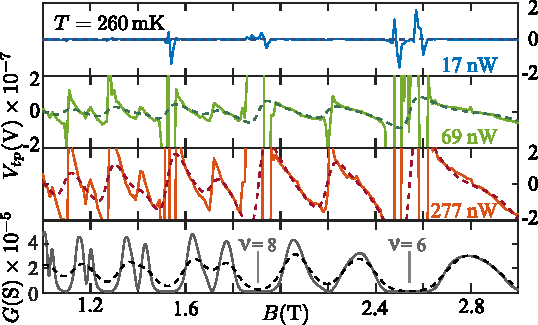
\includegraphics[width=0.7\textwidth]{figures/vtpGmodel/termovoltageConductance/fig3.pdf}
    \caption{Thermovoltage $V_{tp}$  for a fixed temperature and different powers $P^{\prime}$
    applied at the heater, assuming $\Delta T (P^{\prime}) = P^{\prime}/P \; \SI{1.08}{\milli\kelvin}$.
    $P$ and other details are the same as in  Fig.~\ref{fig:lowHifield}.}
    \label{fig:modelHeaterPower}
\end{figure}




\textcolor{red}{METER lo de abajo en el texto anterior}

In the presence of disorder and absence of electron-electron interactions ${\mathcal T}(\varepsilon)$ was originally calculated by Jonson and Girvin \cite{jonson1984thermoelectric}. At high temperatures, electron-phonon interaction gives rise to an additional component to the transport coefficients ${\cal L}_{ij}$. The corresponding thermopower has been studied  in bar geometries for specific filling factors \cite{tieke1996even,zhang2004oscillatory} and, more recently, in illuminated Corbino samples \cite{Zalinge2003}, while no signatures of electron-phonon interaction were found in other experimental works in the Corbino geometry \cite{kobayakawa2013diffusion}.
The thermal conductance has an additional component of purely phononic origin. We have only very limited access to this transport coefficient with the present experimental setup.
